In order to offer a deployment view of our system, we have decided to use the Deployment Diagram. This choice is due to the fact that this diagram is strictly related to the Component Diagram: indeed, it shows how software components, previously described in the Component Diagram, are deployed in hardware. 
\newline
Referring to figure \ref{fig:deployment-diagram}, we have to specify that the web browsers and the Operating Systems supported by our applications, in addiction to the database server, the web server and application server we have chosen, have been already listed in the RASD.\footnote{see the 'Constraints' subsection in the RASD}

\begin{figure}[H]
            \centering
            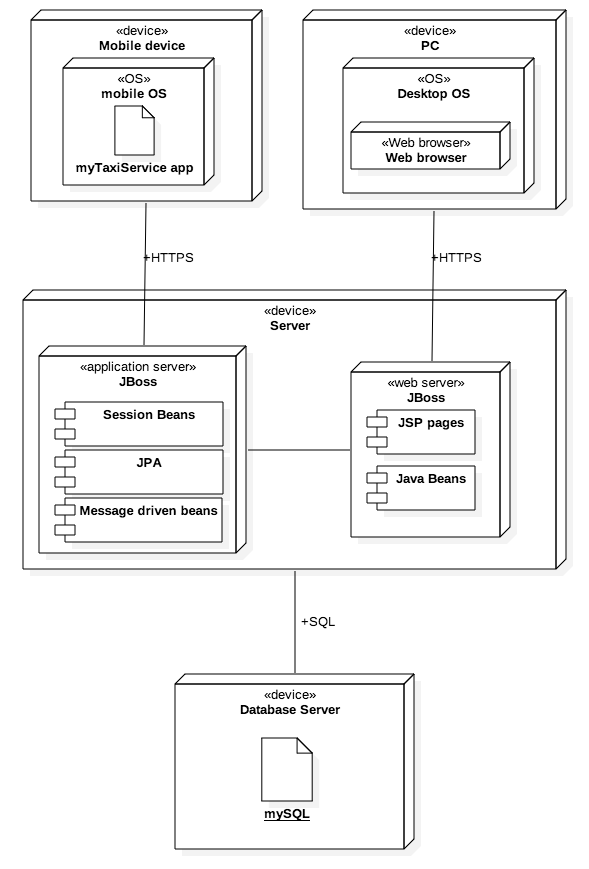
\includegraphics[width=12cm]{./Images/DeploymentDiagram.png}
            \caption{Deployment Diagram}
            \label{fig:deployment-diagram}
\end{figure}
We also give a brief description of the hardware infrastructure. We decided for a dual host configuration: this means that the web server and the application server will be placed on the same machine, while the database will be located on another host. This choice has been preferred to the single host configuration because we want to assure that the data stored in the database are well protected and so, by separating into two hosts, we can put a firewall between them in order to guarantee an higher security.
\newline
Our system will have another firewall in order to filter packets coming from the external network and so it will be placed before the DMZ to protect the internal network.
\begin{figure}[H]
            \centering
            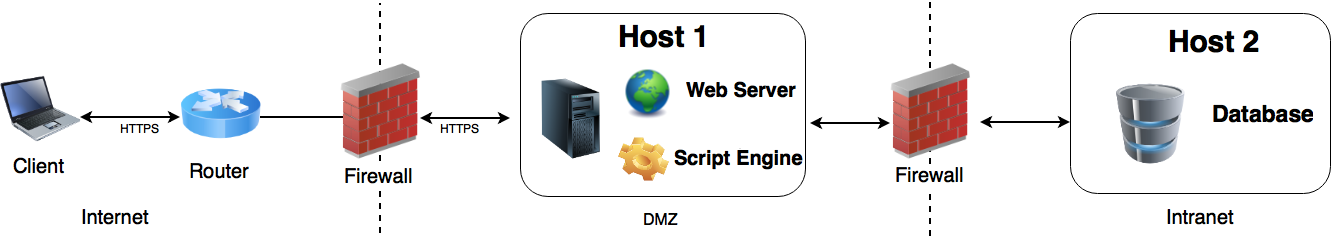
\includegraphics[width=14cm]{./Images/HardwareArchitecture.png}
            \caption{Hardware architecture}
\end{figure}